
%%%%%%%%%%%%%%%%%%%%%%%%%%%%%%%%%%%%%%%%%%%%%%%%%%%%%%%%%%%%%%%%%%%%%%%%%%%%%%%%
%
% Gadget2
%
%%%%%%%%%%%%%%%%%%%%%%%%%%%%%%%%%%%%%%%%%%%%%%%%%%%%%%%%%%%%%%%%%%%%%%%%%%%%%%%%

\section{Simulations with \gadgettwo}
\label{sec:gadget}

%%%%%%%%%%%%%%%%%%%%%%%%%%%%%%%%%%%%%%%%%%%%%%%%%%%%%%%%%%%%%%%%%%%%%%%%%%%%%%%%


We use the massively parallel TreeSPH cosmological \nbody\ simulation code \gadgettwo\ for the dark matter simulations presented in this work.  In this section, we begin with a discussion of the fundamental concepts presented in the original \gadget\ code, then proceed to the improvements made in the \gadgettwo\ code.




%~~~~~~~~~~~~~~~~~~~~~~~~~~~~~~~~~~~~~~~~~~~~~~~~~~~~~~~~~~~~~~~~~~~~~~~~~~~~~~~
\subsection{\gadgettwo}
\label{subsec:gadget--gadget}
%~~~~~~~~~~~~~~~~~~~~~~~~~~~~~~~~~~~~~~~~~~~~~~~~~~~~~~~~~~~~~~~~~~~~~~~~~~~~~~~


Text goes here.



%:::::::::::::::::::::::::::::::::::::::::::::::::::::::::::::::::::::::::::::::
\subsubsection{Gravitational Algorithms}
\label{subsubsec:gadget--gadget--gravitational_algorithms}
%:::::::::::::::::::::::::::::::::::::::::::::::::::::::::::::::::::::::::::::::


Text goes here.

\begin{figure}[t]
	\centering
	\begin{subfigure}{}
		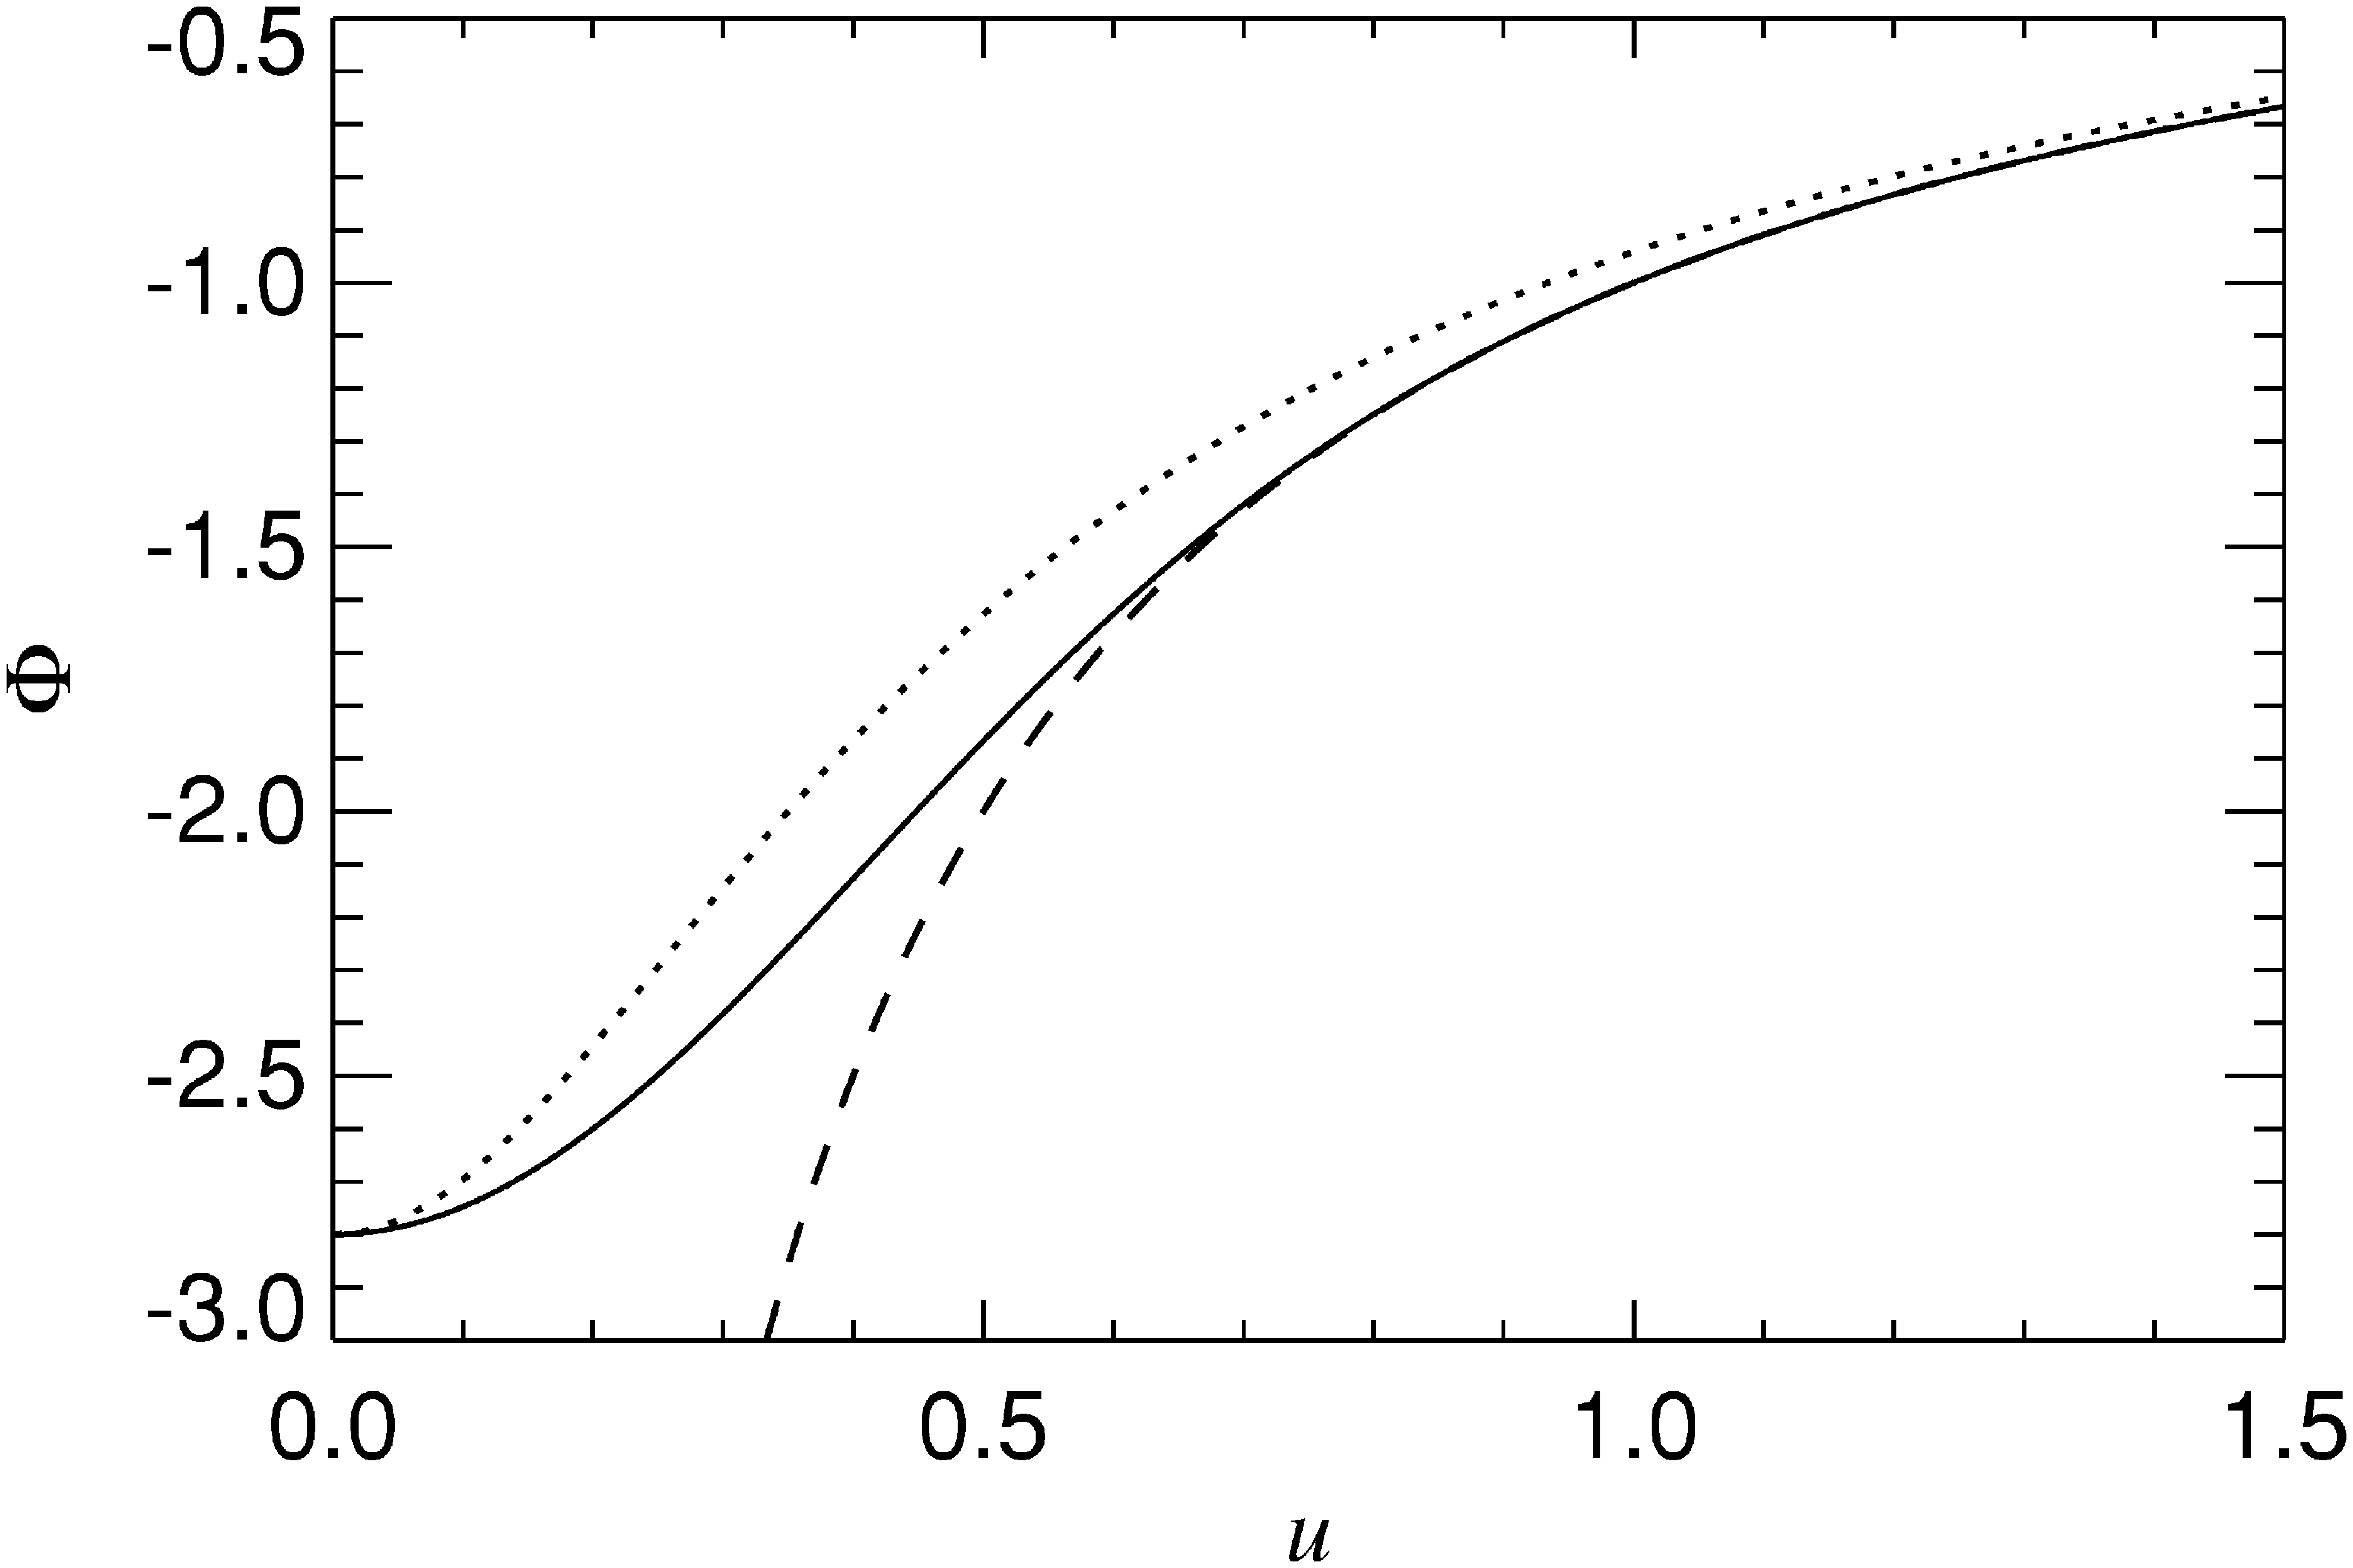
\includegraphics[width=0.48\linewidth]{gadget/softened_potential.eps}
	\end{subfigure}
	~
	\begin{subfigure}{}
		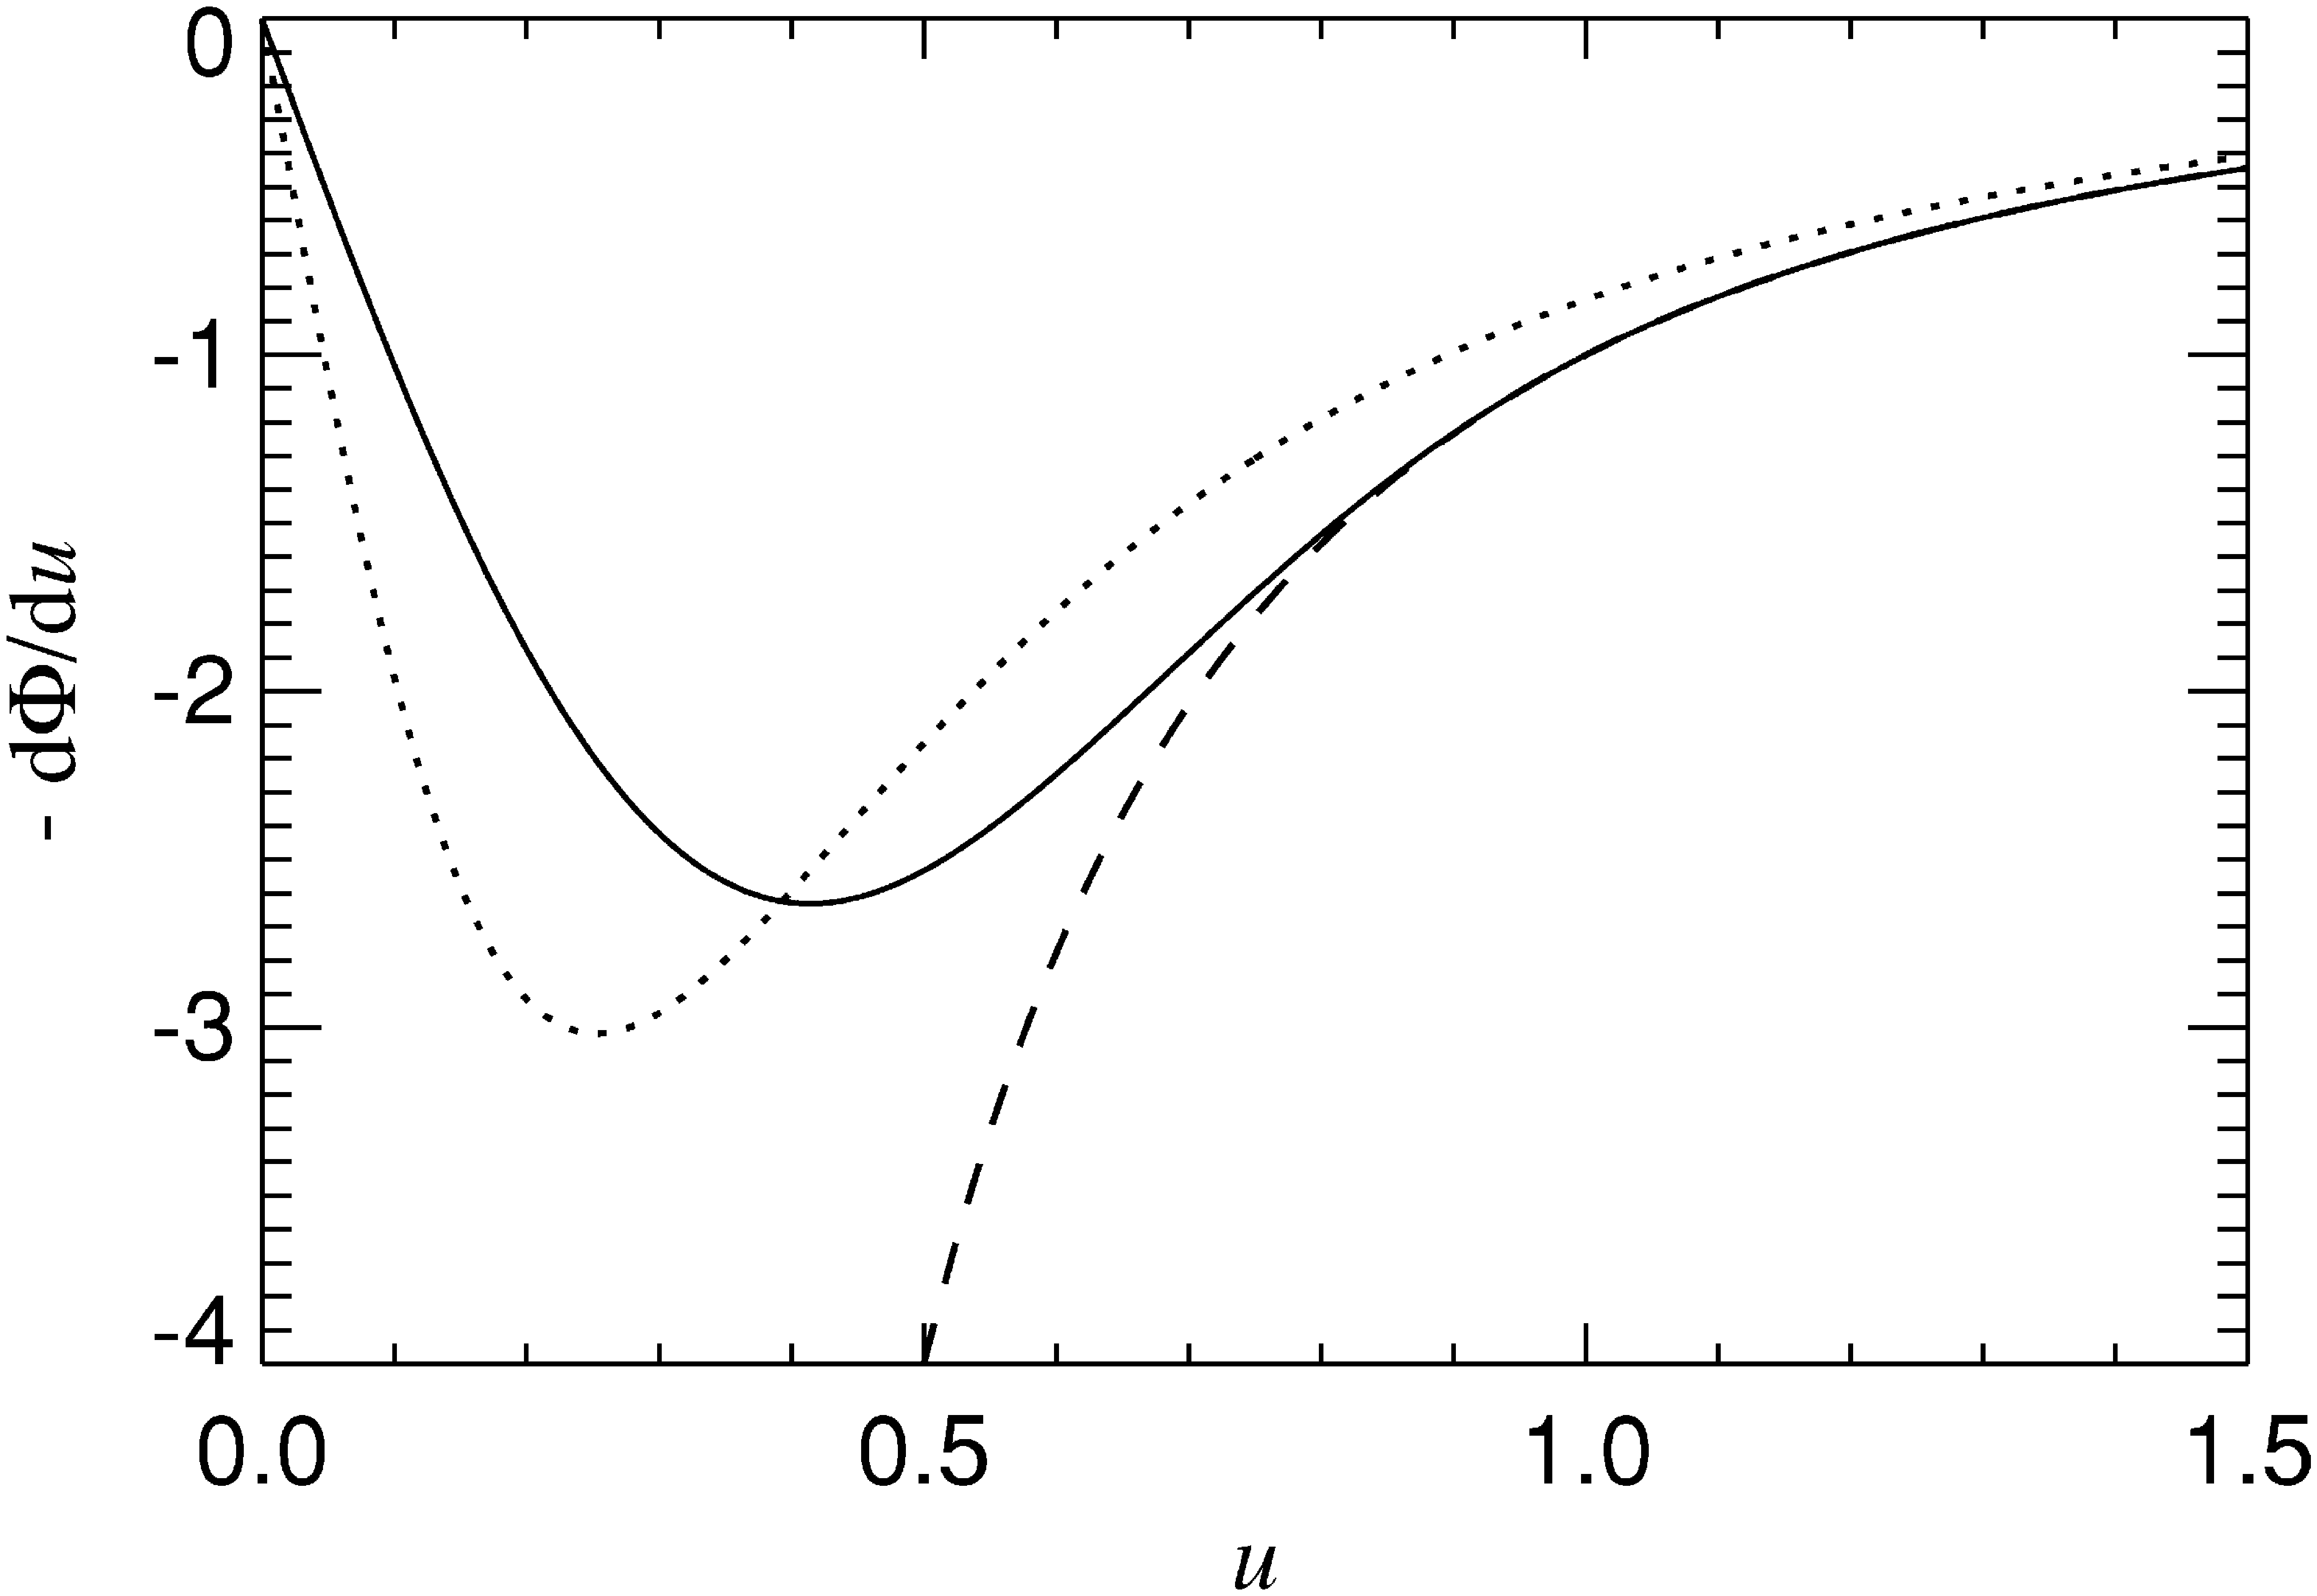
\includegraphics[width=0.48\linewidth]{gadget/softened_force.eps}
	\end{subfigure}
	\caption[Potential and force softening.]{Potential (\emph{left}) and force (\emph{right}) softening.}
	\label{fig:gadget--softening}
\end{figure}

\begin{figure}[t]
	\centering
	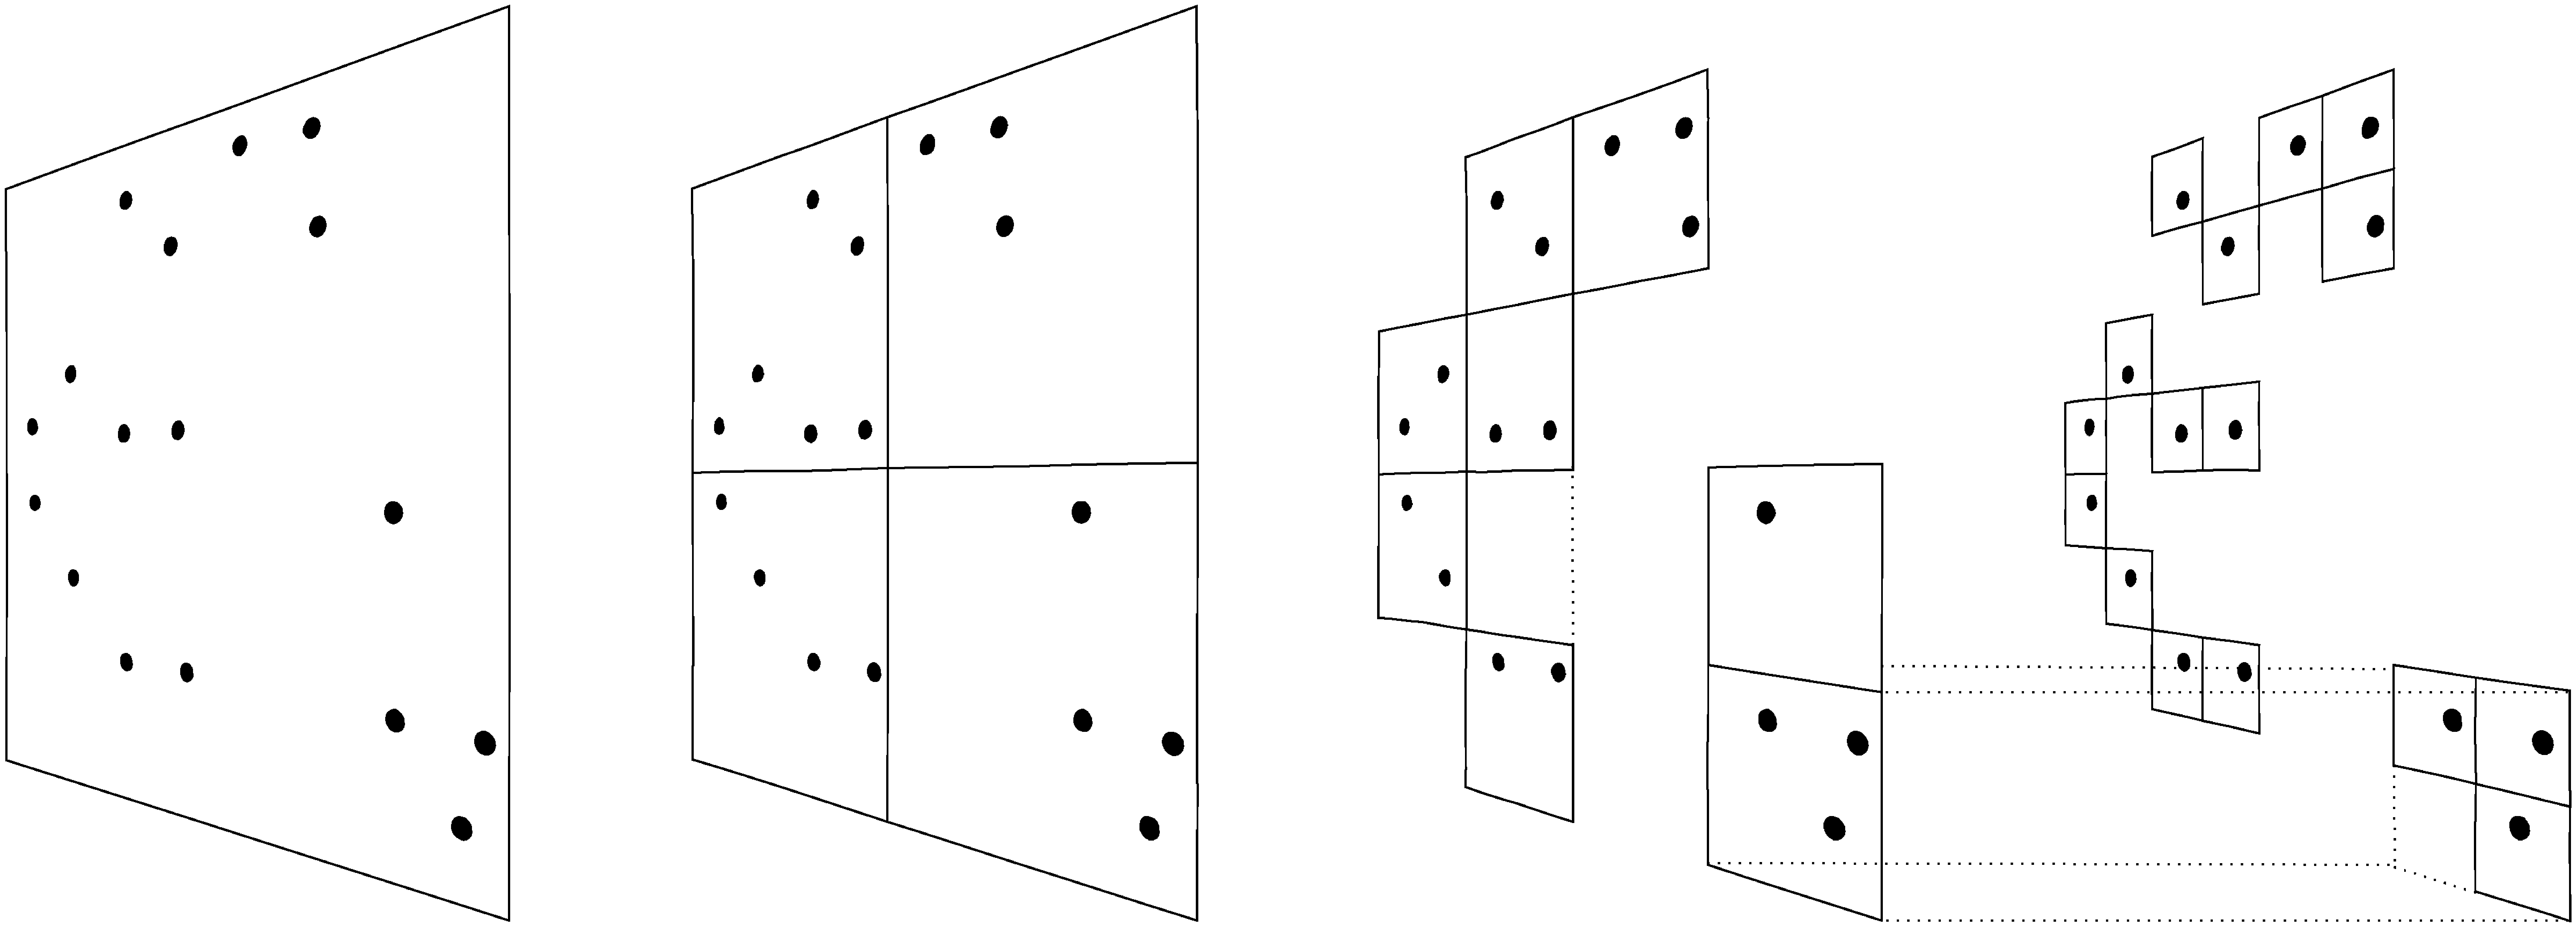
\includegraphics[width=\linewidth]{gadget/tree.eps}
	\caption[Barns-Hut oct-tree in two dimensions.]{Barns-Hut oct-tree in two dimensions.}
	\label{fig:gadget--tree}
\end{figure}



%:::::::::::::::::::::::::::::::::::::::::::::::::::::::::::::::::::::::::::::::
\subsubsection{Time Integration}
\label{subsubsec:gadget--gadget--time_integration}
%:::::::::::::::::::::::::::::::::::::::::::::::::::::::::::::::::::::::::::::::


Text goes here.




%~~~~~~~~~~~~~~~~~~~~~~~~~~~~~~~~~~~~~~~~~~~~~~~~~~~~~~~~~~~~~~~~~~~~~~~~~~~~~~~
\subsection{Simulations}
\label{subsec:gadget--simulations}
%~~~~~~~~~~~~~~~~~~~~~~~~~~~~~~~~~~~~~~~~~~~~~~~~~~~~~~~~~~~~~~~~~~~~~~~~~~~~~~~


Text goes here.




